% Options for packages loaded elsewhere
% Options for packages loaded elsewhere
\PassOptionsToPackage{unicode}{hyperref}
\PassOptionsToPackage{hyphens}{url}
\PassOptionsToPackage{dvipsnames,svgnames,x11names}{xcolor}
%
\documentclass[
  letterpaper,
  DIV=11,
  numbers=noendperiod]{scrreprt}
\usepackage{xcolor}
\usepackage[margin=0.5in]{geometry}
\usepackage{amsmath,amssymb}
\setcounter{secnumdepth}{-\maxdimen} % remove section numbering
\usepackage{iftex}
\ifPDFTeX
  \usepackage[T1]{fontenc}
  \usepackage[utf8]{inputenc}
  \usepackage{textcomp} % provide euro and other symbols
\else % if luatex or xetex
  \usepackage{unicode-math} % this also loads fontspec
  \defaultfontfeatures{Scale=MatchLowercase}
  \defaultfontfeatures[\rmfamily]{Ligatures=TeX,Scale=1}
\fi
\usepackage{lmodern}
\ifPDFTeX\else
  % xetex/luatex font selection
\fi
% Use upquote if available, for straight quotes in verbatim environments
\IfFileExists{upquote.sty}{\usepackage{upquote}}{}
\IfFileExists{microtype.sty}{% use microtype if available
  \usepackage[]{microtype}
  \UseMicrotypeSet[protrusion]{basicmath} % disable protrusion for tt fonts
}{}
\makeatletter
\@ifundefined{KOMAClassName}{% if non-KOMA class
  \IfFileExists{parskip.sty}{%
    \usepackage{parskip}
  }{% else
    \setlength{\parindent}{0pt}
    \setlength{\parskip}{6pt plus 2pt minus 1pt}}
}{% if KOMA class
  \KOMAoptions{parskip=half}}
\makeatother
% Make \paragraph and \subparagraph free-standing
\makeatletter
\ifx\paragraph\undefined\else
  \let\oldparagraph\paragraph
  \renewcommand{\paragraph}{
    \@ifstar
      \xxxParagraphStar
      \xxxParagraphNoStar
  }
  \newcommand{\xxxParagraphStar}[1]{\oldparagraph*{#1}\mbox{}}
  \newcommand{\xxxParagraphNoStar}[1]{\oldparagraph{#1}\mbox{}}
\fi
\ifx\subparagraph\undefined\else
  \let\oldsubparagraph\subparagraph
  \renewcommand{\subparagraph}{
    \@ifstar
      \xxxSubParagraphStar
      \xxxSubParagraphNoStar
  }
  \newcommand{\xxxSubParagraphStar}[1]{\oldsubparagraph*{#1}\mbox{}}
  \newcommand{\xxxSubParagraphNoStar}[1]{\oldsubparagraph{#1}\mbox{}}
\fi
\makeatother


\usepackage{longtable,booktabs,array}
\usepackage{calc} % for calculating minipage widths
% Correct order of tables after \paragraph or \subparagraph
\usepackage{etoolbox}
\makeatletter
\patchcmd\longtable{\par}{\if@noskipsec\mbox{}\fi\par}{}{}
\makeatother
% Allow footnotes in longtable head/foot
\IfFileExists{footnotehyper.sty}{\usepackage{footnotehyper}}{\usepackage{footnote}}
\makesavenoteenv{longtable}
\usepackage{graphicx}
\makeatletter
\newsavebox\pandoc@box
\newcommand*\pandocbounded[1]{% scales image to fit in text height/width
  \sbox\pandoc@box{#1}%
  \Gscale@div\@tempa{\textheight}{\dimexpr\ht\pandoc@box+\dp\pandoc@box\relax}%
  \Gscale@div\@tempb{\linewidth}{\wd\pandoc@box}%
  \ifdim\@tempb\p@<\@tempa\p@\let\@tempa\@tempb\fi% select the smaller of both
  \ifdim\@tempa\p@<\p@\scalebox{\@tempa}{\usebox\pandoc@box}%
  \else\usebox{\pandoc@box}%
  \fi%
}
% Set default figure placement to htbp
\def\fps@figure{htbp}
\makeatother


% definitions for citeproc citations
\NewDocumentCommand\citeproctext{}{}
\NewDocumentCommand\citeproc{mm}{%
  \begingroup\def\citeproctext{#2}\cite{#1}\endgroup}
\makeatletter
 % allow citations to break across lines
 \let\@cite@ofmt\@firstofone
 % avoid brackets around text for \cite:
 \def\@biblabel#1{}
 \def\@cite#1#2{{#1\if@tempswa , #2\fi}}
\makeatother
\newlength{\cslhangindent}
\setlength{\cslhangindent}{1.5em}
\newlength{\csllabelwidth}
\setlength{\csllabelwidth}{3em}
\newenvironment{CSLReferences}[2] % #1 hanging-indent, #2 entry-spacing
 {\begin{list}{}{%
  \setlength{\itemindent}{0pt}
  \setlength{\leftmargin}{0pt}
  \setlength{\parsep}{0pt}
  % turn on hanging indent if param 1 is 1
  \ifodd #1
   \setlength{\leftmargin}{\cslhangindent}
   \setlength{\itemindent}{-1\cslhangindent}
  \fi
  % set entry spacing
  \setlength{\itemsep}{#2\baselineskip}}}
 {\end{list}}
\usepackage{calc}
\newcommand{\CSLBlock}[1]{\hfill\break\parbox[t]{\linewidth}{\strut\ignorespaces#1\strut}}
\newcommand{\CSLLeftMargin}[1]{\parbox[t]{\csllabelwidth}{\strut#1\strut}}
\newcommand{\CSLRightInline}[1]{\parbox[t]{\linewidth - \csllabelwidth}{\strut#1\strut}}
\newcommand{\CSLIndent}[1]{\hspace{\cslhangindent}#1}



\setlength{\emergencystretch}{3em} % prevent overfull lines

\providecommand{\tightlist}{%
  \setlength{\itemsep}{0pt}\setlength{\parskip}{0pt}}



 


\KOMAoption{captions}{tableheading}
\makeatletter
\@ifpackageloaded{caption}{}{\usepackage{caption}}
\AtBeginDocument{%
\ifdefined\contentsname
  \renewcommand*\contentsname{Table of contents}
\else
  \newcommand\contentsname{Table of contents}
\fi
\ifdefined\listfigurename
  \renewcommand*\listfigurename{List of Figures}
\else
  \newcommand\listfigurename{List of Figures}
\fi
\ifdefined\listtablename
  \renewcommand*\listtablename{List of Tables}
\else
  \newcommand\listtablename{List of Tables}
\fi
\ifdefined\figurename
  \renewcommand*\figurename{Figure}
\else
  \newcommand\figurename{Figure}
\fi
\ifdefined\tablename
  \renewcommand*\tablename{Table}
\else
  \newcommand\tablename{Table}
\fi
}
\@ifpackageloaded{float}{}{\usepackage{float}}
\floatstyle{ruled}
\@ifundefined{c@chapter}{\newfloat{codelisting}{h}{lop}}{\newfloat{codelisting}{h}{lop}[chapter]}
\floatname{codelisting}{Listing}
\newcommand*\listoflistings{\listof{codelisting}{List of Listings}}
\makeatother
\makeatletter
\makeatother
\makeatletter
\@ifpackageloaded{caption}{}{\usepackage{caption}}
\@ifpackageloaded{subcaption}{}{\usepackage{subcaption}}
\makeatother
\usepackage{bookmark}
\IfFileExists{xurl.sty}{\usepackage{xurl}}{} % add URL line breaks if available
\urlstyle{same}
\hypersetup{
  pdftitle={The Werewolf Among Us: Humans vs LLMs in Multi-Agent Games},
  pdfauthor={Bhavana Jonnalagadda; Riley Jones},
  pdfkeywords={social deduction games, persuasion modeling, Werewolf
Among Us dataset, large language models, multimodal analysis},
  colorlinks=true,
  linkcolor={blue},
  filecolor={Maroon},
  citecolor={Blue},
  urlcolor={Blue},
  pdfcreator={LaTeX via pandoc}}


\title{The Werewolf Among Us: Humans vs LLMs in Multi-Agent Games}
\author{Bhavana Jonnalagadda \and Riley Jones}
\date{2025-05-05}
\begin{document}
\maketitle
\begin{abstract}
Abstract TODO
\end{abstract}

\renewcommand*\contentsname{Table of contents}
{
\hypersetup{linkcolor=}
\setcounter{tocdepth}{2}
\tableofcontents
}

\chapter{Introduction}\label{introduction}

\begin{itemize}
\tightlist
\item
  A description of the problem and its significance
\item
  How do LLMs function in a multi-agent environment?

  \begin{itemize}
  \tightlist
  \item
    Each has limited information
  \item
    Approximately the same ability, traits, skills
  \end{itemize}
\item
  We use LLMs to simulate whether synthetic agents can participate in
  complex, adversarial group dynamics
\item
  Werewolf is a good candiate for testing multi agent systems of
  cooperation and secrecy

  \begin{itemize}
  \tightlist
  \item
    Need citation
  \item
    The game tests adaptive reasoning, strategic alignment, and
    collective threat detection under special conditions
  \end{itemize}
\end{itemize}

\section{Related Work}\label{related-work}

\subsection{Multi-Agent LLMs}\label{multi-agent-llms}

\begin{itemize}
\tightlist
\item
  Among us game (\citeproc{ref-chiAMONGAGENTSEvaluatingLarge2024}{Chi,
  Mao, and Tang 2024})
\item
  Collective problem solving
  (\citeproc{ref-duLargeLanguageModels2024}{Du, Rajivan, and Gonzalez
  2024})

  \begin{itemize}
  \tightlist
  \item
    ``analyses indicate that LLM agent groups exhibit more
    disagreements, complex statements, and a propensity for positive
    statements compared to human groups''
  \end{itemize}
\item
  Govsim (\citeproc{ref-piattiCooperateCollapseEmergence2024}{Piatti et
  al. 2024})

  \begin{itemize}
  \tightlist
  \item
    ``In GOVSIM, a society of AI agents must collectively balance
    exploiting a common resource with sustaining it for future use. This
    environment enables the study of how ethical considerations,
    strategic planning, and negotiation skills impact cooperative
    outcomes.''
  \end{itemize}
\item
  All found similar themes

  \begin{itemize}
  \tightlist
  \item
    That LLMs are capable and good at understanding the rules
  \item
    That they can cooperate and be sneaky
  \end{itemize}
\end{itemize}

\subsection{LLMs and Werewolf}\label{llms-and-werewolf}

\begin{itemize}
\tightlist
\item
  Examination of improving werewolf by LLMs
  (\citeproc{ref-xuLanguageAgentsReinforcement2024}{Xu et al. 2024})

  \begin{itemize}
  \tightlist
  \item
    ``our agents use an LLM to perform deductive reasoning and generate
    a diverse set of action candidates. Then an RL policy trained to
    optimize the decision-making ability chooses an action from the
    candidates to play in the game. Extensive experiments show that our
    agents overcome the intrinsic bias and outperform existing LLM-based
    agents in the Werewolf game.''
  \end{itemize}
\item
  Werewolf Arena (\citeproc{ref-bailisWerewolfArenaCase2024}{Bailis,
  Friedhoff, and Chen 2024})

  \begin{itemize}
  \tightlist
  \item
    Used in this paper
  \end{itemize}
\item
  Explicitly discuss how none of the exisiting LLM+Werewolf papers
  examine the differences/compare from a human dataset
\end{itemize}

\chapter{Methods}\label{methods}

\section{Data}\label{data}

\subsection{Werewolf Among Us Human
Dataset}\label{werewolf-among-us-human-dataset}

\begin{itemize}
\tightlist
\item
  Human dataset description
  (\citeproc{ref-laiWerewolfUsMultimodal2022}{Lai et al. 2022})
\item
  Is specifically for a form of one-night werewolf

  \begin{itemize}
  \tightlist
  \item
    Describe key differences
  \end{itemize}
\item
  Used specifically for the text available

  \begin{itemize}
  \tightlist
  \item
    and annotations of persuasion strategy on the text
  \end{itemize}
\end{itemize}

\subsection{Werewolf Arena}\label{werewolf-arena}

\begin{itemize}
\tightlist
\item
  (\citeproc{ref-bailisWerewolfArenaCase2024}{Bailis, Friedhoff, and
  Chen 2024})
\item
  Discuss the framework, how it works, prompts, etc
\item
  Discuss what types of runs we did
\item
  Discuss the data included in output
\item
  Talk about how we had to annotate the LLM speech with persuasion
  strategies ourselves
\end{itemize}

\section{Analysis}\label{analysis}

\begin{itemize}
\tightlist
\item
  Formatted data to match, performed various comparisons
\end{itemize}

\chapter{Results}\label{results}

\begin{figure}[H]

\centering{

\centering{

\begin{verbatim}
Unable to display output for mime type(s): text/html
\end{verbatim}

}

\subcaption{\label{fig-llm-winrounds-1}The LLM wins, by how many rounds
that partiticular game had.}

\centering{

\pandocbounded{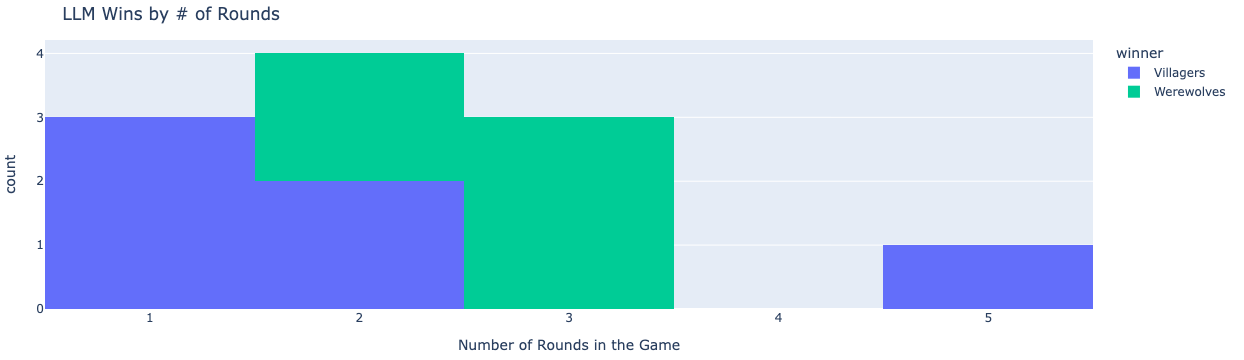
\includegraphics[keepaspectratio]{paper_files/figure-latex/Data-EDA_Comparison-fig-llm-winrounds-output-2.png}}

}

\subcaption{\label{fig-llm-winrounds-2}}

}

\caption{\label{fig-llm-winrounds}}

\end{figure}%

\textsubscript{Source:
\href{https://CUBoulder-DS.github.io/CSCI-5423-Final/Data/EDA_Comparison-preview.html\#cell-fig-llm-winrounds}{Werewolf
Among Us: Human vs LLM Analysis}}

\begin{figure}[H]

\centering{

\pandocbounded{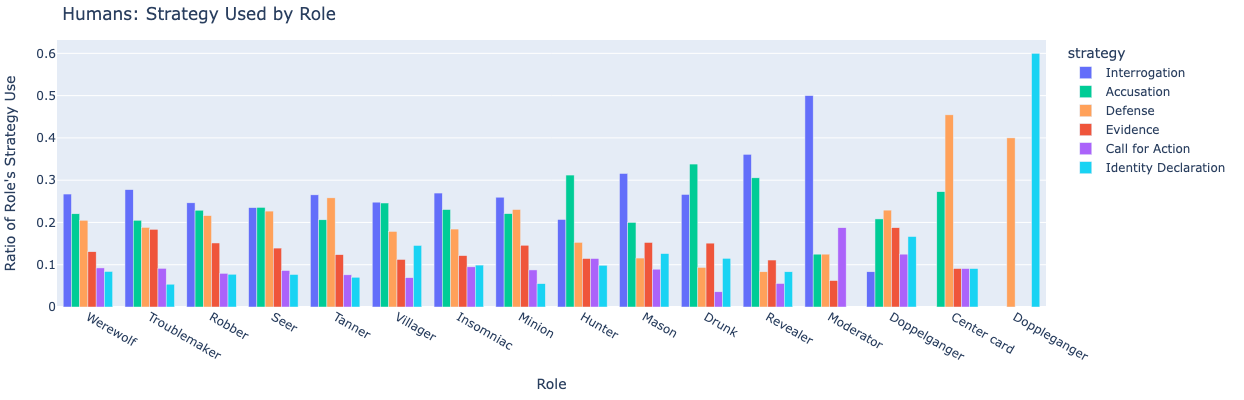
\includegraphics[keepaspectratio]{paper_files/figure-latex/Data-EDA_Comparison-fig-stratbyrole-hum-output-1.png}}

}

\caption{\label{fig-stratbyrole-hum}}

\end{figure}%

\textsubscript{Source:
\href{https://CUBoulder-DS.github.io/CSCI-5423-Final/Data/EDA_Comparison-preview.html\#cell-fig-stratbyrole-hum}{Werewolf
Among Us: Human vs LLM Analysis}}

\begin{figure}[H]

\centering{

\pandocbounded{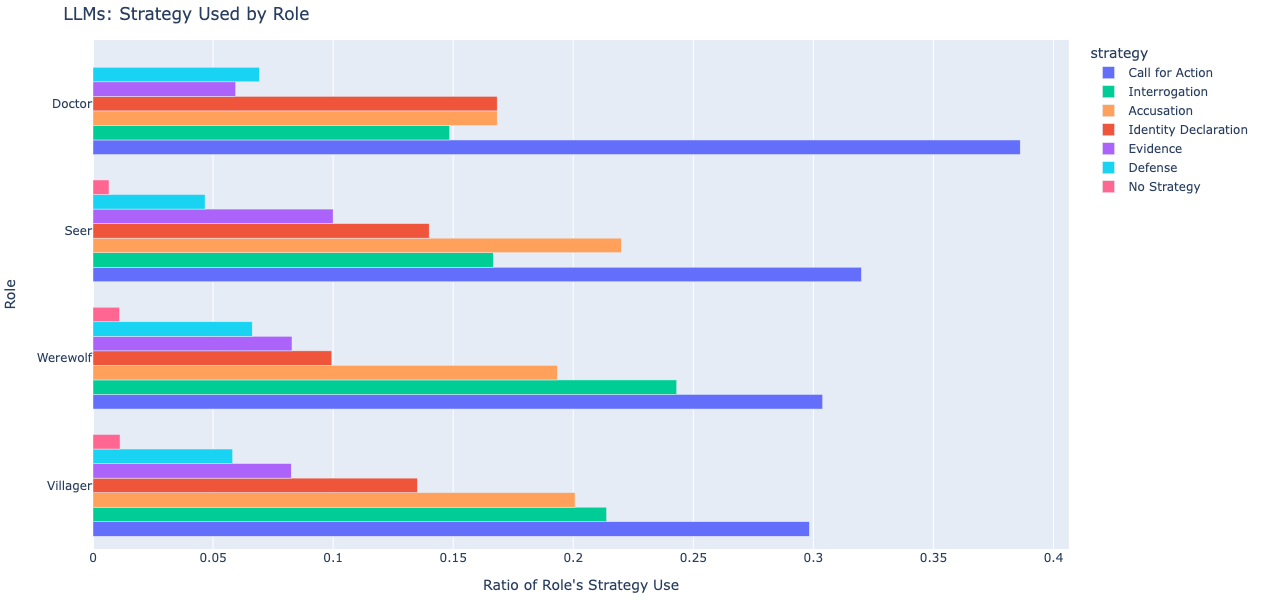
\includegraphics[keepaspectratio]{paper_files/figure-latex/Data-EDA_Comparison-fig-stratbyrole-llms-output-1.png}}

}

\caption{\label{fig-stratbyrole-llms}}

\end{figure}%

\textsubscript{Source:
\href{https://CUBoulder-DS.github.io/CSCI-5423-Final/Data/EDA_Comparison-preview.html\#cell-fig-stratbyrole-llms}{Werewolf
Among Us: Human vs LLM Analysis}}

\chapter{Discussion and Conclusion}\label{discussion-and-conclusion}

Interpret findings, discuss limitations, and propose future work.

\section{Limitations}\label{limitations}

\section{Future Work}\label{future-work}

\section{Summary}\label{summary}

Summarize contributions and insights from the project.

\begin{center}\rule{0.5\linewidth}{0.5pt}\end{center}

\chapter{References}\label{references}

\phantomsection\label{refs}
\begin{CSLReferences}{1}{0}
\bibitem[\citeproctext]{ref-bailisWerewolfArenaCase2024}
Bailis, Suma, Jane Friedhoff, and Feiyang Chen. 2024. {``Werewolf
{Arena}: {A Case Study} in {LLM Evaluation} via {Social Deduction}.''}
July 18, 2024. \url{https://doi.org/10.48550/arXiv.2407.13943}.

\bibitem[\citeproctext]{ref-chiAMONGAGENTSEvaluatingLarge2024}
Chi, Yizhou, Lingjun Mao, and Zineng Tang. 2024. {``{AMONGAGENTS}:
{Evaluating Large Language Models} in the {Interactive Text-Based Social
Deduction Game}.''} July 24, 2024.
\url{https://doi.org/10.48550/arXiv.2407.16521}.

\bibitem[\citeproctext]{ref-choRoundTableInvestigatingGroup2024}
Cho, Young-Min, Raphael Shu, Nilaksh Das, Tamer Alkhouli, Yi-An Lai,
Jason Cai, Monica Sunkara, and Yi Zhang. 2024. {``{RoundTable}:
{Investigating Group Decision-Making Mechanism} in {Multi-Agent
Collaboration}.''} November 11, 2024.
\url{https://doi.org/10.48550/arXiv.2411.07161}.

\bibitem[\citeproctext]{ref-duLargeLanguageModels2024}
Du, Yinuo, Prashanth Rajivan, and Cleotilde Gonzalez. 2024. {``Large
{Language Models} for {Collective Problem-Solving}: {Insights} into
{Group Consensus Decision-Making}.''} \emph{Proceedings of the Annual
Meeting of the Cognitive Science Society} 46 (0).
\url{https://escholarship.org/uc/item/6s060914}.

\bibitem[\citeproctext]{ref-laiWerewolfUsMultimodal2022}
Lai, Bolin, Hongxin Zhang, Miao Liu, Aryan Pariani, Fiona Ryan, Wenqi
Jia, Shirley Anugrah Hayati, James M. Rehg, and Diyi Yang. 2022.
{``Werewolf {Among Us}: {A Multimodal Dataset} for {Modeling Persuasion
Behaviors} in {Social Deduction Games}.''} December 16, 2022.
\url{https://doi.org/10.48550/arXiv.2212.08279}.

\bibitem[\citeproctext]{ref-piattiCooperateCollapseEmergence2024}
Piatti, Giorgio, Zhijing Jin, Max Kleiman-Weiner, Bernhard Schölkopf,
Mrinmaya Sachan, and Rada Mihalcea. 2024. {``Cooperate or {Collapse}:
{Emergence} of {Sustainable Cooperation} in a {Society} of {LLM
Agents}.''} \emph{Advances in Neural Information Processing Systems} 37
(December): 111715--59.
\url{https://proceedings.neurips.cc/paper_files/paper/2024/hash/ca9567d8ef6b2ea2da0d7eed57b933ee-Abstract-Conference.html}.

\bibitem[\citeproctext]{ref-xuLanguageAgentsReinforcement2024}
Xu, Zelai, Chao Yu, Fei Fang, Yu Wang, and Yi Wu. 2024. {``Language
{Agents} with {Reinforcement Learning} for {Strategic Play} in the
{Werewolf Game}.''} February 20, 2024.
\url{https://doi.org/10.48550/arXiv.2310.18940}.

\end{CSLReferences}

\begin{center}\rule{0.5\linewidth}{0.5pt}\end{center}

\chapter{Project Contributions}\label{project-contributions}

\textbf{Bhavana Jonnalagadda}:

\begin{itemize}
\tightlist
\item
  Paper framework (Quarto) setup
\item
  Github repo management
\item
  EDA on LLM dataset
\item
  Final comparison EDA and results analysis
\item
  Results section
\item
  Discussion and Conclusion section
\item
  Abstract
\end{itemize}

\textbf{Riley Jones}:

\begin{itemize}
\tightlist
\item
  EDA on human dataset
\item
  Werewolf Arena LLM simulation running and data aquisition
\item
  Introduction section
\item
  Methods section
\end{itemize}




\end{document}
